\documentclass[11pt]{article}
\usepackage[preprint]{acl}
\usepackage{amsmath}

% Standard package includes
\usepackage{times}
\usepackage{latexsym}

% For proper rendering and hyphenation of words containing Latin characters (including in bib files)
\usepackage[T1]{fontenc}

% This assumes your files are encoded as UTF8
\usepackage[utf8]{inputenc}

% This is not strictly necessary, and may be commented out,
% but it will improve the layout of the manuscript,
% and will typically save some space.
\usepackage{microtype}

% This is also not strictly necessary, and may be commented out.
% However, it will improve the aesthetics of text in
% the typewriter font.
\usepackage{inconsolata}

\usepackage{graphicx}
\usepackage{booktabs}
\usepackage{xcolor}
\graphicspath{{part1_behavioral/report/figures/}}
\definecolor{battle}{HTML}{2A78D6}
\definecolor{vac}{HTML}{EB6834}

\title{Investigating the influence of geography on LLM decision-making in ambiguous contexts}

\author{Hoffmann Muki \\
  \texttt{hoffmuki@umd.edu} \\\And
  Pritika Ramu \\
  \texttt{pramu@umd.edu} \\}

\begin{document}
\maketitle
% \begin{abstract}
% \emph{1 paragraph}
% \end{abstract}

\section{Introduction}

% TAKEAWAY: LLMs are used to code conflict events, and descriptions often leave the deciding fact open, so context can enter the decision.
Large language models (LLMs) offer a low-cost means of annotating text for social science research \citep{gilardi-etal-2023-chatgpt}. In conflict-event coding, protests are distinguished from riots by whether demonstrators use violence, and battles from attacks on civilians by the organization and combat capabilities of the actors involved \citep{acled-codebook}. An event description, however, may leave precisely these facts unresolved. In such cases, a model's classification may depend on contextual cues as well as the actions explicitly described.

% TAKEAWAY: Our question is whether the country alone changes the class, and we name the phenomenon without presuming it is an error.
We investigate whether the country named in an otherwise identical description changes an LLM's preference between two event classes. Such dependence matters because comparisons across countries based on model annotations could reflect geographic assumptions as well as differences in the reported events. Our focus is on two classification boundaries: Protest versus Riot (PR), and Battle versus Violence against civilians (BV). We use \emph{country sensitivity} to describe changes in class preference induced by the country substitution; detecting this sensitivity alone cannot distinguish the use of contextual base rates from stereotyping or establish a coding error.

% TAKEAWAY: We answer it with a large factorial dataset in which the country is the only manipulated variable, measured against placebo names and in both option orders.
Building on BBQ's evaluation of responses to under-informative contexts \citep{parrish-etal-2022-bbq}, we construct 3,520 event descriptions whose evidence comes from acts attested in ACLED event notes, and which vary systematically in evidence, sentence frame, wording, actors, grievances, places and times. Each description is rendered with no country, with 37 real countries and with 20 invented placebo names, and Llama-3.2-3B-Instruct labels every rendering with the class options in both orders (408,320 prompts). The placebo names estimate how much a label moves when any name is inserted, so country sensitivity is the part that exceeds them. This report presents the behavioral measurement; it identifies the descriptions and countries that a subsequent mechanistic analysis will examine.

\section{Related Work}

\citet{gilardi-etal-2023-chatgpt} find that zero-shot ChatGPT outperforms crowd workers on several annotation tasks involving tweets and news articles. Their findings motivate our application, while our matched design examines sensitivity to geographic context that aggregate annotation accuracy does not capture.

\citet{parrish-etal-2022-bbq} introduce BBQ, which contrasts under-informative and disambiguated contexts to examine whether social stereotypes influence question answering. We extend its evaluation of ambiguous contexts to country substitutions in event coding, measuring relative class preference in a binary task without an ``unknown'' option.

\citet{manvi-etal-2024-geographically} document geographic biases in LLM predictions, including associations between socioeconomic conditions and subjective ratings of locations. Our study examines whether a geographic cue also changes the classification of an event whose reported circumstances remain fixed. \citet{yin-etal-2022-geomlama} introduce GeoMLAMA to probe geographically diverse commonsense knowledge across countries and languages. Their benchmark motivates our distinction between country sensitivity and coding error, since the appropriate commonsense answer can vary by location.

\citet{zheng-etal-2024-selectors} show that multiple-choice decisions are sensitive to option order and identify biases associated with the tokens used to identify options \citep[see also][]{zhao-etal-2021-calibrate,pezeshkpour-hruschka-2024-large}. We therefore present every prompt in both option orders and report the model's letter preference separately from country effects.

\section{Method}

\subsection{Evidence items from ACLED}

% TAKEAWAY: The evidence in every description is something human coders actually encounter, and its position on the evidence scale is measured from their decisions, not chosen by us.
\paragraph{Items and evidence scale.}
We draw evidence from 137,947 ACLED events with free-text notes (five regional exports, October 2024 to October 2025; \citealp{raleigh-etal-2010-acled}). A fixed lexicon of regular expressions identifies concrete acts in the notes, such as throwing stones, burning tires or carrying a pistol, and every act attested in at least 20 notes becomes an evidence item: 29 for PR and 22 for BV. Each item's position on the evidence scale is $P(\text{higher}\mid\text{act})$, the share of attesting notes that ACLED coders assigned to the more severe class (Riot or Battle). It ranges from 0.01 (burning an effigy) to 1.00 (throwing a petrol bomb) for PR, and from 0.09 (the other group were fishermen) to 0.92 (a member of the other group threw a grenade) for BV. One anchor at each end of each boundary states the class unambiguously and serves as a competence check.

% TAKEAWAY: Item sentences are written so the model must infer the class from the act itself.
\paragraph{Item sentences.}
Each item is written as one factual sentence of 5--16 words. Automated checks require that it contain no hedge or modal, share no word stem with the class names or definitions, name no entity, and use no outcome or casualty term. The model therefore has to reason from the described act, not from vocabulary borrowed from the class definitions.

\subsection{Factorial design}

% TAKEAWAY: Descriptions vary systematically along every dimension of wording and context, so a country effect can be separated from the phrasing of any single description.
\paragraph{Factors.}
Every description combines one item with a sentence frame (2 per boundary), a wording of the item sentence (2, related by fixed lexical substitutions such as \emph{threw} $\rightarrow$ \emph{hurled}) and a context (16 per boundary). PR contexts form a $4\times4$ Latin square of actors and grievances, in which each of four places occurs once with every actor and once with every grievance; BV contexts cross four places with four times of day. Both designs are balanced, so each context factor is estimated independently of the others, and each context is assigned to one of two halves that provide an internal replication. The design yields 3,520 descriptions (1,984 PR, 1,536 BV).

% TAKEAWAY: The country phrase is the only thing that changes between conditions, and this is verified for every text.
\paragraph{Country slot.}
The country enters as a single phrase, ``in \textit{Country}'', directly after the place (Figure~\ref{fig:example}). Each description is rendered under 58 name conditions, giving 204,160 texts, and the build verifies for every text that deleting the phrase recovers the no-country description exactly.

\subsection{Countries and placebo names}

% TAKEAWAY: Real countries span every region; placebo names give the baseline that any inserted name produces.
We use 37 real countries covering every world region, inserted in their natural English form (``the United States''). As a baseline we generate 20 placebo names from a fixed syllable inventory with a fixed seed, rejecting any candidate that matches an ACLED place name, a world country or a single vocabulary token, and matching the character-length distribution of the real names. A placebo name estimates how far a label moves because a name of that length was inserted; country sensitivity is the movement beyond this range. We also record each name's token count as a covariate.

\subsection{Measurement}

% TAKEAWAY: The model's choice is read directly from the probabilities of the two answer letters, one prompt at a time.
\paragraph{Decision score.}
The model receives the definitions of both classes, the two options labelled A and B, and an instruction to answer with one letter (Appendix~\ref{sec:prompts}). At the first answer position we read $\log P(\text{A})$ and $\log P(\text{B})$, both single tokens that together carry essentially all of the probability mass. For description $i$, name $c$ and option order $o$,
\begin{equation}
d_{ico}=\log P(\ell^{+}_{o}\mid x_{ico})-\log P(\ell^{-}_{o}\mid x_{ico}),
\end{equation}
where $\ell^{+}_{o}$ is the letter of the higher class (Riot or Battle) in order $o$. Positive values favour the higher class. Each prompt is scored in its own forward pass, without batching.

% TAKEAWAY: Two complementary labels separate the model's underlying judgement from the answer a user would receive in one fixed order.
\paragraph{Two orders, two labels.}
Order A lists one class first and order B reverses the options and their definitions. The \emph{order-averaged score} $s_{ic}=(d_{icA}+d_{icB})/2$ cancels any additive preference for a letter or position, and gives the \emph{averaged label}: the higher class if $s_{ic}>m$, the lower class if $s_{ic}<-m$, and near-boundary otherwise, with $m=0.5$ nats. The \emph{strict label} requires the same answer in both orders, $d_{icA}$ and $d_{icB}$ both beyond $\pm m$, and otherwise marks the pair as order-dependent. The averaged label measures the model's judgement; the strict label asks whether the answer survives a change of option order. We report the model's letter preference, $\log P(\text{A})-\log P(\text{B})$ averaged over orders, alongside both.

\subsection{Analysis}

% TAKEAWAY: Every comparison is made against placebo names within the same description, with a pre-specified plan.
A description \emph{flips} if at least one real country assigns the higher class and at least one the lower class. We compare the flip rate of 20 real countries (averaged over 500 random subsets) with that of the 20 placebo names, so both sets have equal size. A country's effect is its mean shift relative to the placebo mean for the same description, $\Delta_{ic}=s_{ic}-\bar{s}_{i,\text{placebo}}$, averaged over descriptions. We fit $s_{ic}=\alpha_i+\beta_c+\varepsilon_{ic}$ separately for real and placebo names and report the share of within-description variance explained by the name, and we correlate country effects estimated on the two context halves. Intervals are 95\% bootstrap intervals over descriptions (2,000 resamples). The analysis was specified before results were examined; two robustness checks added afterwards (leave-one-country-out flip rates and effects among single-token names) are marked as such.

\section{Experimental Details}

% TAKEAWAY: One model, one prompt per boundary, selected on anchors only.
\paragraph{Model and prompts.}
We evaluate Llama-3.2-3B-Instruct (revision \texttt{0cb88a4f76}, bf16) with its standard chat template and a fixed date header. Each boundary uses one task prompt with class definitions, chosen from four paraphrases by a criterion fixed before any country condition was scored: correct labels for every anchor, in both orders and both frames, on a separate set of pilot contexts, with $P(\text{A})+P(\text{B})\geq0.9$. The selected prompts meet it with anchor accuracy 1.0.

% TAKEAWAY: The run is complete, deterministic and released.
\paragraph{Compute and data.}
All 408,320 prompts were scored on one RTX A4000 (about 4.3 hours); rescoring a sample on a second GPU of the same type reproduced every score exactly. We release the descriptions with all factor levels, one row per description and name with both order scores and both labels, and a per-description summary listing which countries assign which label.

\section{Intermediate Results}

\begin{figure}[t]
\centering
\small
\fbox{\parbox{0.95\columnwidth}{\raggedright
\textit{System:} \ldots\ \textbf{Battle}: a fight between organized armed sides, each capable of hurting the other. \textbf{Violence against civilians}: an organized armed group purposely harms unarmed civilians who are unable to protect themselves. A.~Battle \ B.~Violence against civilians. Give your answer as one letter.\\[3pt]
\textit{User:} A shooting at dawn on a coastal road \textbf{in \underline{\hspace{1.4em}?\hspace{1.4em}}} involved members of an armed group and members of another group. Members of the other group were truck drivers waiting by the road.}}\\[4pt]
{\footnotesize\setlength{\tabcolsep}{3.5pt}\begin{tabular}{@{}lcccl@{}}
\toprule
 & \multicolumn{2}{c}{$P(\text{Battle})$} & & \\
Country & order A & order B & $s$ & Label \\
\midrule
United States & 0.25 & 0.93 & $+0.75$ & \textcolor{battle}{\textbf{Battle}} \\
United Kingdom & 0.20 & 0.93 & $+0.63$ & \textcolor{battle}{\textbf{Battle}} \\
\emph{no country} & 0.18 & 0.75 & $-0.19$ & near boundary \\
\emph{Gaor} (placebo) & 0.15 & 0.85 & $\phantom{+}0.00$ & near boundary \\
Bangladesh & 0.13 & 0.68 & $-0.56$ & \textcolor{vac}{\textbf{VAC}} \\
Pakistan & 0.11 & 0.62 & $-0.81$ & \textcolor{vac}{\textbf{VAC}} \\
\bottomrule
\end{tabular}}
\caption{A description whose label depends on the country (BV, item \emph{drivers}, ACLED $P(\text{Battle}\mid\text{act})=0.17$). Only the country phrase changes. In both orders the model favours letter B, so $P(\text{Battle})$ is low in order A (Battle = A) and high in order B (Battle = B); the order-averaged score $s$ removes this preference, and its label is shown. 2 real countries assign Battle and 12 assign Violence against civilians (VAC); all 20 placebo names stay near the boundary.}
\label{fig:example}
\end{figure}

\begin{figure*}[t]
\centering
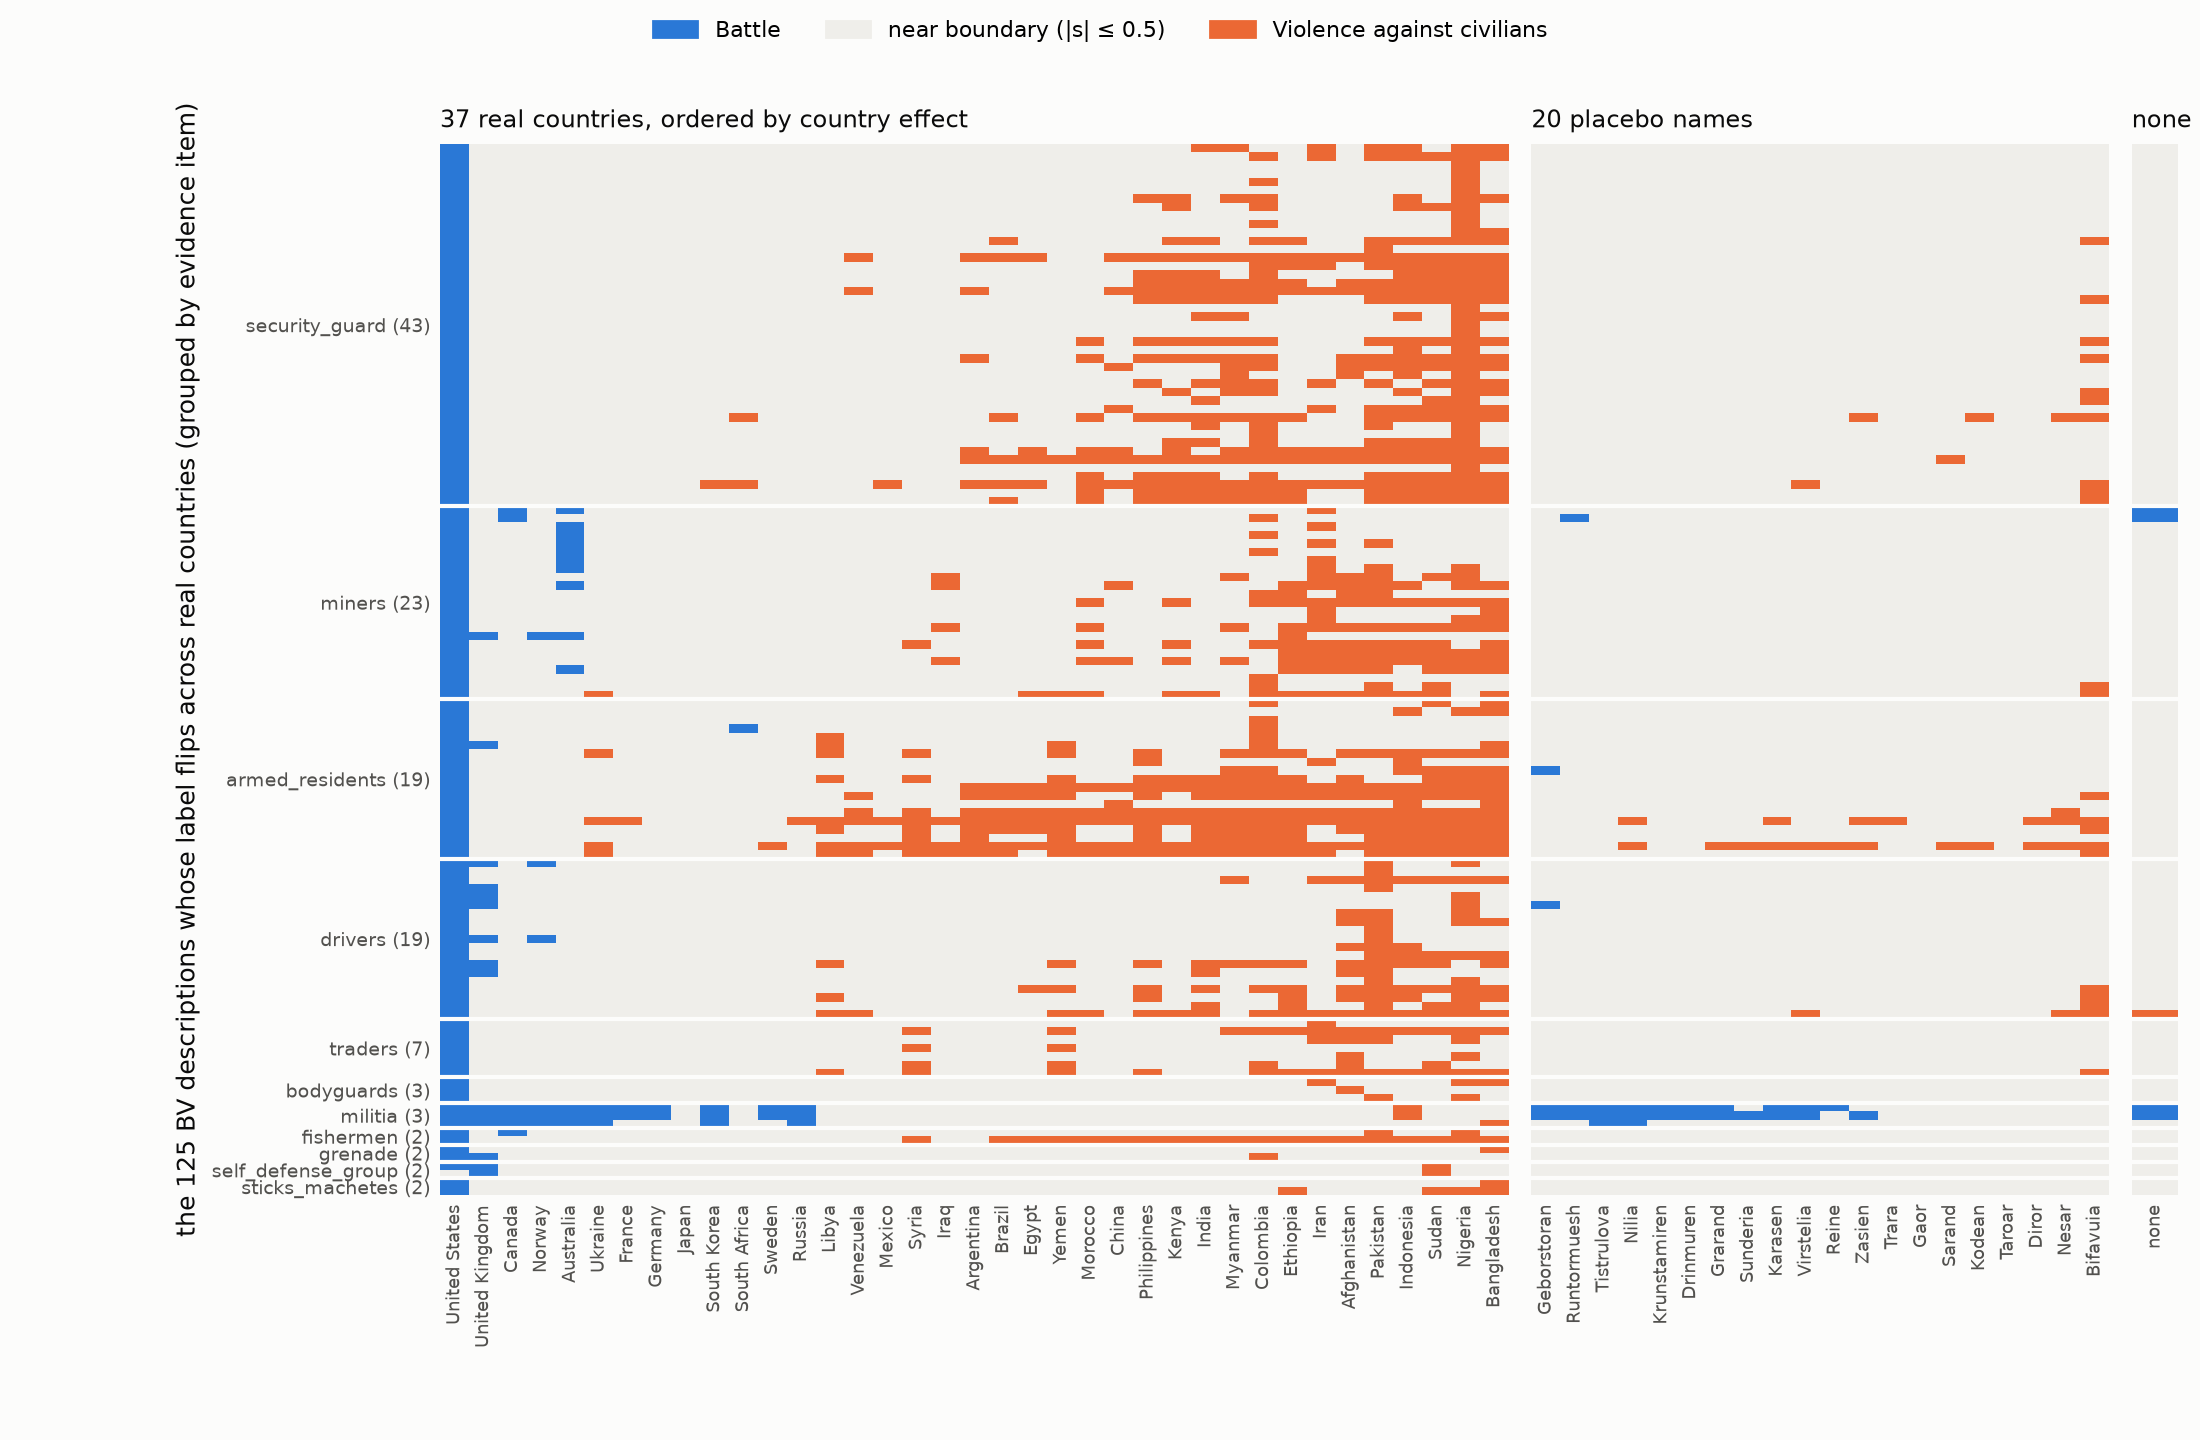
\includegraphics[width=\textwidth]{fig7_flip_matrix.png}
\caption{Every BV description whose averaged label flips across real countries (125 of 1,536; rows, grouped by evidence item) under every name (columns: 37 real countries ordered by country effect, 20 placebo names, no country). Within a row only the country changes. Real countries assign both labels in the same row, in a consistent order; placebo names never do.}
\label{fig:matrix}
\end{figure*}

% TAKEAWAY: The measurement is sound, but the model has a strong letter preference, so the order-averaged score is the right scale for country effects.
\paragraph{Measurement validity.}
In all 408,320 prompts the top token is A or B (5th percentile of $P(\text{A})+P(\text{B})$: 0.9999 for PR, 0.9994 for BV), and the averaged label is correct for every anchor under every name condition. The model also prefers one answer letter by about 1.1 nats: A in PR (98\% of description--name pairs) and B in BV (98\%). As a result the strict label is order-dependent for 41\% of PR pairs and 82\% of BV pairs, while the order-averaged score cancels the preference by construction. Country effects are therefore measured on $s$.

% TAKEAWAY: Evidence drives most of the decision; country effects operate within a narrower band, and matter most where the model reads the evidence as balanced.
\paragraph{Evidence determines most of the score.}
PR labels follow the ACLED evidence scale for most items, with one systematic departure: burning an effigy, a flag or documents is labelled Riot, although ACLED coders assign these acts to Riot in at most 10\% of notes, consistent with a literal reading of ``damaging property'' in the definition. For BV, the model separates the classes when the description states whether the other group could fight back (unarmed victims, returned fire), and scores within about one nat of the boundary when the evidence is a weapon or an identity alone (a pistol, armed residents, miners, drivers). These near-boundary items are where a country effect can decide the label.

% TAKEAWAY: For BV, the country shifts the model's judgement systematically, far beyond what placebo names produce, in a consistent geographic order.
\paragraph{BV: strong, ordered country sensitivity.}
Country effects on BV are 3.6 times as dispersed as placebo effects (SD 0.23 vs.\ 0.065 nats), and the name explains 65\% of within-description variance for real countries against 28\% for placebo names (Table~\ref{tab:effects}). The ordering is consistent: descriptions set in the United States ($+0.59$), the United Kingdom ($+0.42$), Canada, Norway and Australia (each $+0.22$ to $+0.24$) move toward Battle, and those set in Bangladesh ($-0.44$), Nigeria, Sudan, Indonesia and Pakistan ($-0.33$ to $-0.39$) toward Violence against civilians. The effect is not a property of name length: among the 32 single-token countries the SD remains 0.19 nats (robustness check).

% TAKEAWAY: The shift changes the actual label for a meaningful share of BV descriptions, where placebo names never do.
\paragraph{BV: the country changes the label.}
In 8.1\% of BV descriptions (95\% CI 6.8--9.6\%) real countries assign both labels; with 20 countries, size-matched to the placebo set, the rate is 3.9\% (3.2--4.5\%), and placebo names never flip a description (Figures~\ref{fig:example} and~\ref{fig:matrix}). Flips concentrate on items the model reads as balanced: a security guard among the victims (67\% of its descriptions), miners (36\%), drivers and armed residents (30\% each). The United States is on the Battle side of 124 of the 125 flips; leaving it out, 1.8\% of descriptions still flip, while the Violence-against-civilians side is shared by many countries, led by Nigeria (84 descriptions), Pakistan (68) and Bangladesh (65).

% TAKEAWAY: PR is the contrast case: country sensitivity there is no larger than placebo sensitivity.
\paragraph{PR: country effects at placebo level.}
For PR, real countries explain no more within-description variance than placebo names (27\% vs.\ 28\%), and only 0.45\% of descriptions flip in the size-matched comparison (placebo: 0.05\%). The main common feature is that a real country name moves the score slightly toward Protest relative to an invented name (by 0.10 nats on average). The same model, prompt format and pipeline thus produce a strong country effect on one boundary and essentially none on the other.

% TAKEAWAY: The effects are stable properties of the names; the placebo comparison, not replication alone, is what identifies them as country effects.
\paragraph{Replication and order.}
Country effects estimated on disjoint halves of the contexts agree closely (BV $r>0.99$, PR $r=0.98$). Placebo effects replicate equally well, so each name carries a stable effect of its own and the comparison with placebos is what identifies a country effect. Under the strict label no description flips on either boundary: the letter preference (about 1.1 nats) exceeds every country effect, so the country decides the model's judgement only within the range that the order swap leaves open.

\begin{table}[t]
\centering
\small
\begin{tabular}{@{}lcc@{}}
\toprule
 & PR & BV \\
\midrule
SD of effects, real (placebo) & 0.11 (0.09) & 0.23 (0.07) \\
Variance explained, real (placebo) & 27\% (28\%) & 65\% (28\%) \\
Real countries outside placebo range & 10/37 & 25/37 \\
Flip rate, 20 real (size-matched) & 0.45\% & 3.86\% \\
Flip rate, 20 placebo & 0.05\% & 0\% \\
Flip rate, 37 real & 0.86\% & 8.14\% \\
Split-half $r$, real & 0.98 & $>$0.99 \\
\bottomrule
\end{tabular}
\caption{Country sensitivity relative to placebo names (order-averaged score, nats; flips at $m=0.5$).}
\label{tab:effects}
\end{table}

\section{Discussion and Next Steps}

% TAKEAWAY: The design works: holding everything but the country fixed, with a placebo baseline, isolates country sensitivity and shows it is specific to one boundary.
\paragraph{What the design establishes.}
Holding the description fixed and comparing real countries to placebo names separates country sensitivity from the general effect of inserting a name, and the balanced factorial design shows that the effect is not tied to particular phrasings or contexts. The result is specific: a strong, geographically ordered effect for Battle versus Violence against civilians, decisive where the evidence leaves open whether the victims could fight back, and none beyond placebo level for Protest versus Riot.

% TAKEAWAY: What the results do not yet show, stated as the open questions the next phase addresses.
\paragraph{Open questions.}
Country sensitivity is not by itself a coding error: the BV ordering is consistent with the model drawing on beliefs about where organized armed conflict or one-sided violence is common, as well as with stereotyping, and the present data cannot separate the two. Placebo names control for the presence and length of a name but not for its familiarity, so part of what distinguishes a real country may be frequency rather than geography. The letter preference is large relative to country effects, which makes the order-averaged score essential and the strict label conservative; whether other prompts and models share the same country ordering remains to be tested.

% TAKEAWAY: The next steps follow directly from these questions.
\paragraph{Next steps.}
\begin{enumerate}
\itemsep0em
\item \textbf{Why the country matters.} Integrated gradients \citep{sundararajan-etal-2017-axiomatic} on the order-averaged logit difference for near-boundary BV descriptions, attributing each description with a country and with a placebo. Predictions are fixed in advance: if the model reads the country as evidence about whether the victims could fight back, attribution to the country should be largest where the evidence sentence is least informative (security guard, miners, drivers) and smallest where it is decisive (unarmed, returned fire).
\item \textbf{Familiarity control.} Add real but rarely mentioned places and familiar non-country names to separate familiarity from geography.
\item \textbf{Generality.} Repeat the measurement with Qwen3.5-4B and with a second task paraphrase per boundary.
\item \textbf{Held-out replication.} Re-estimate country effects on reserved context values before any further design decision.
\item \textbf{Human reference.} Collect human labels for a sample of descriptions so that the evidence scale carries human judgements as well as ACLED frequencies.
\end{enumerate}

\bibliography{custom}

\appendix

\section{Task Prompts}
\label{sec:prompts}

System prompts in order A; order B reverses the two definitions and the two options. The user turn is the event description.

\paragraph{PR.}
\begin{small}
\begin{verbatim}
You code demonstration events for a conflict-event
dataset. Read the event description and decide which
of the two event types below it is.

Protest: a public demonstration in which participants
remain nonviolent, including demonstrations that face
intervention or violence from others.

Riot: a demonstration in which participants engage in
violence or destruction, such as attacking people or
damaging property.

A. Protest
B. Riot

Answer with one letter: A or B.
\end{verbatim}
\end{small}

\paragraph{BV.}
\begin{small}
\begin{verbatim}
Below is a short report of a violent incident. Assign
it to one of the two event types used in conflict
monitoring that are listed below.

Battle: a fight between organized armed sides, each
capable of hurting the other.

Violence against civilians: an organized armed group
purposely harms unarmed civilians who are unable to
protect themselves.

A. Battle
B. Violence against civilians

Give your answer as one letter: A or B.
\end{verbatim}
\end{small}

\section{Additional Figures}

\begin{figure*}[t]
\centering
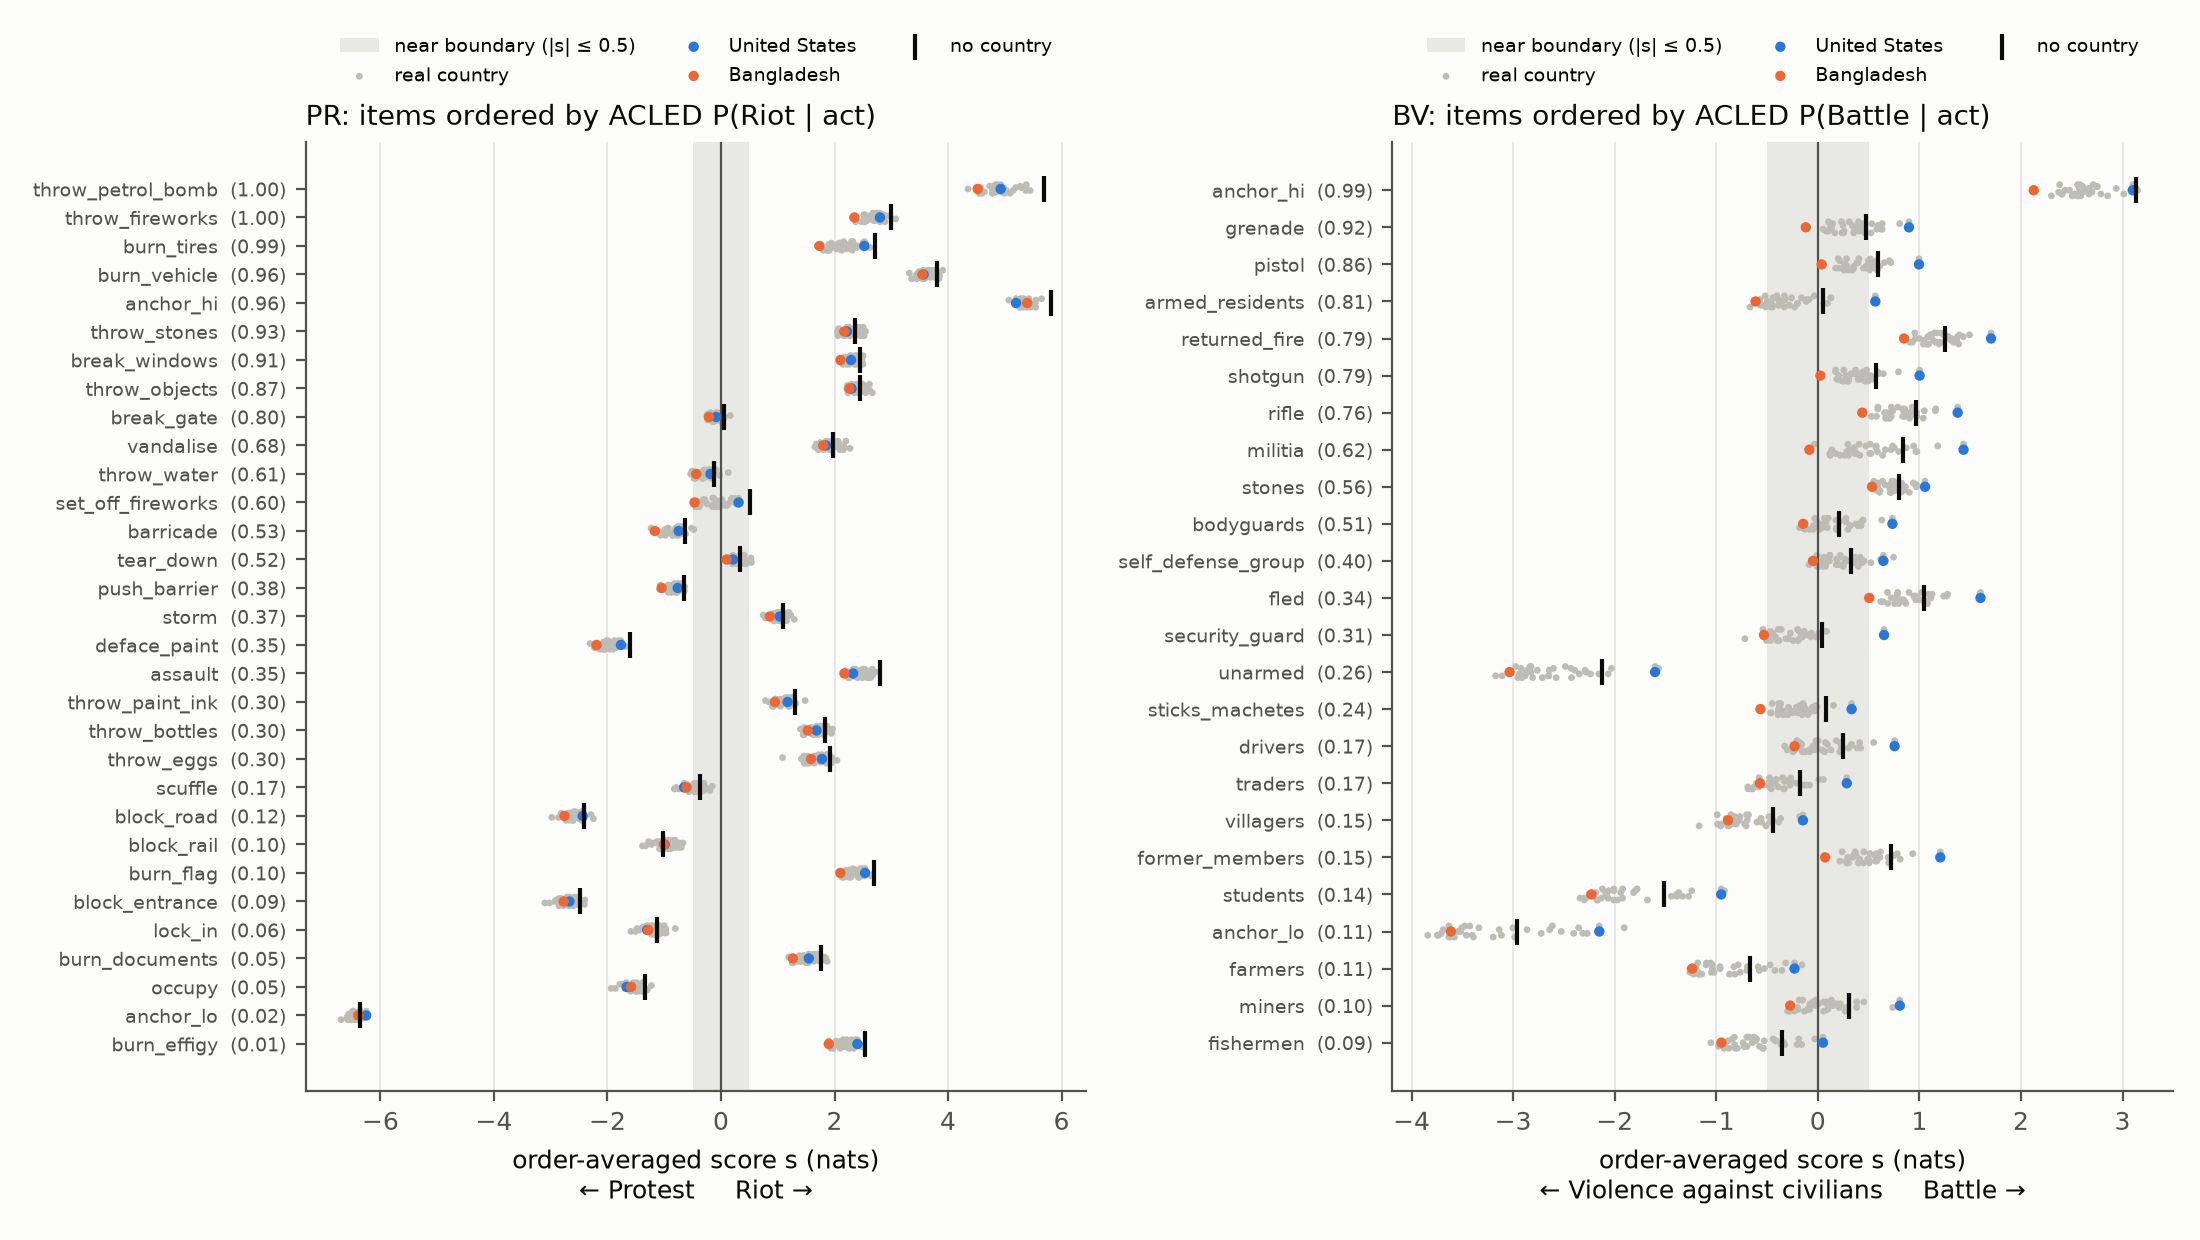
\includegraphics[width=\textwidth]{fig3_ladder_averaged.png}
\caption{Order-averaged score by evidence item, items ordered by ACLED $P(\text{higher}\mid\text{act})$. Grey: each real country's mean over the item's 64 descriptions; blue: the United States; orange: Bangladesh; black tick: no country; shaded band: near boundary.}
\label{fig:ladder}
\end{figure*}

\begin{figure*}[t]
\centering
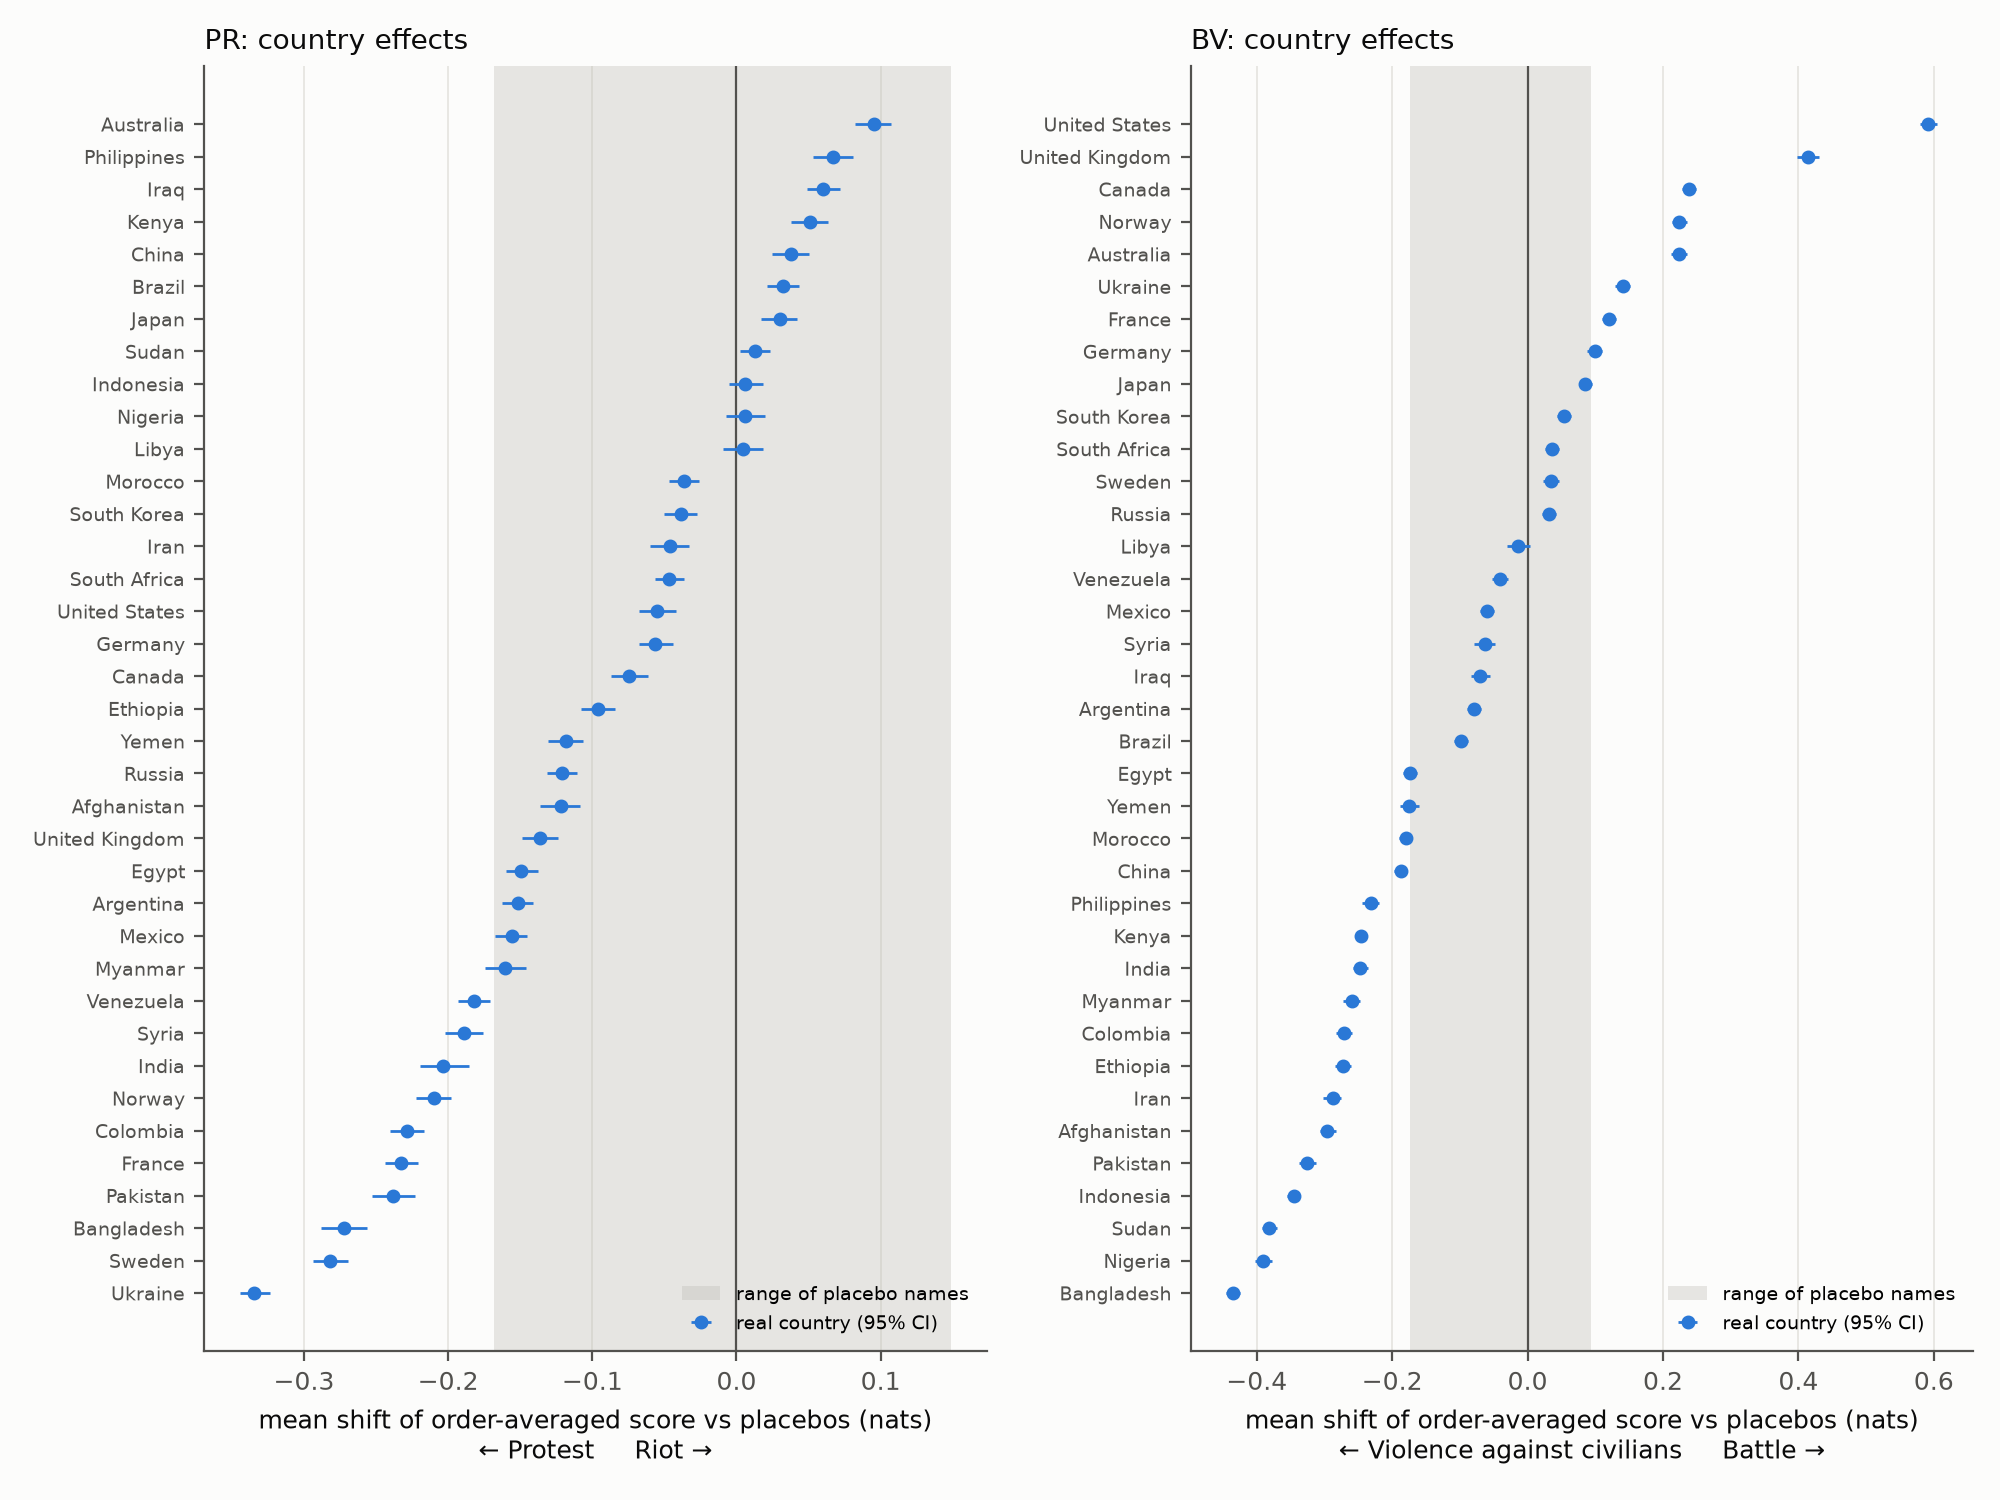
\includegraphics[width=0.85\textwidth]{fig5_country_effects.png}
\caption{Country effects: mean shift of the order-averaged score relative to the placebo mean, with 95\% bootstrap intervals. The shaded band spans the placebo names' own effects.}
\label{fig:effects}
\end{figure*}

\end{document}
